% !TeX root = ../main.tex

\chapter{系统详细设计与实现}

\section{流水线管理}
% 流水线管理主要包含对流水线中各个子概念及其操作的封装。类图如图\ref{fig:流水线管理类图}所示。
% \begin{figure}[h]
%   \centering
%   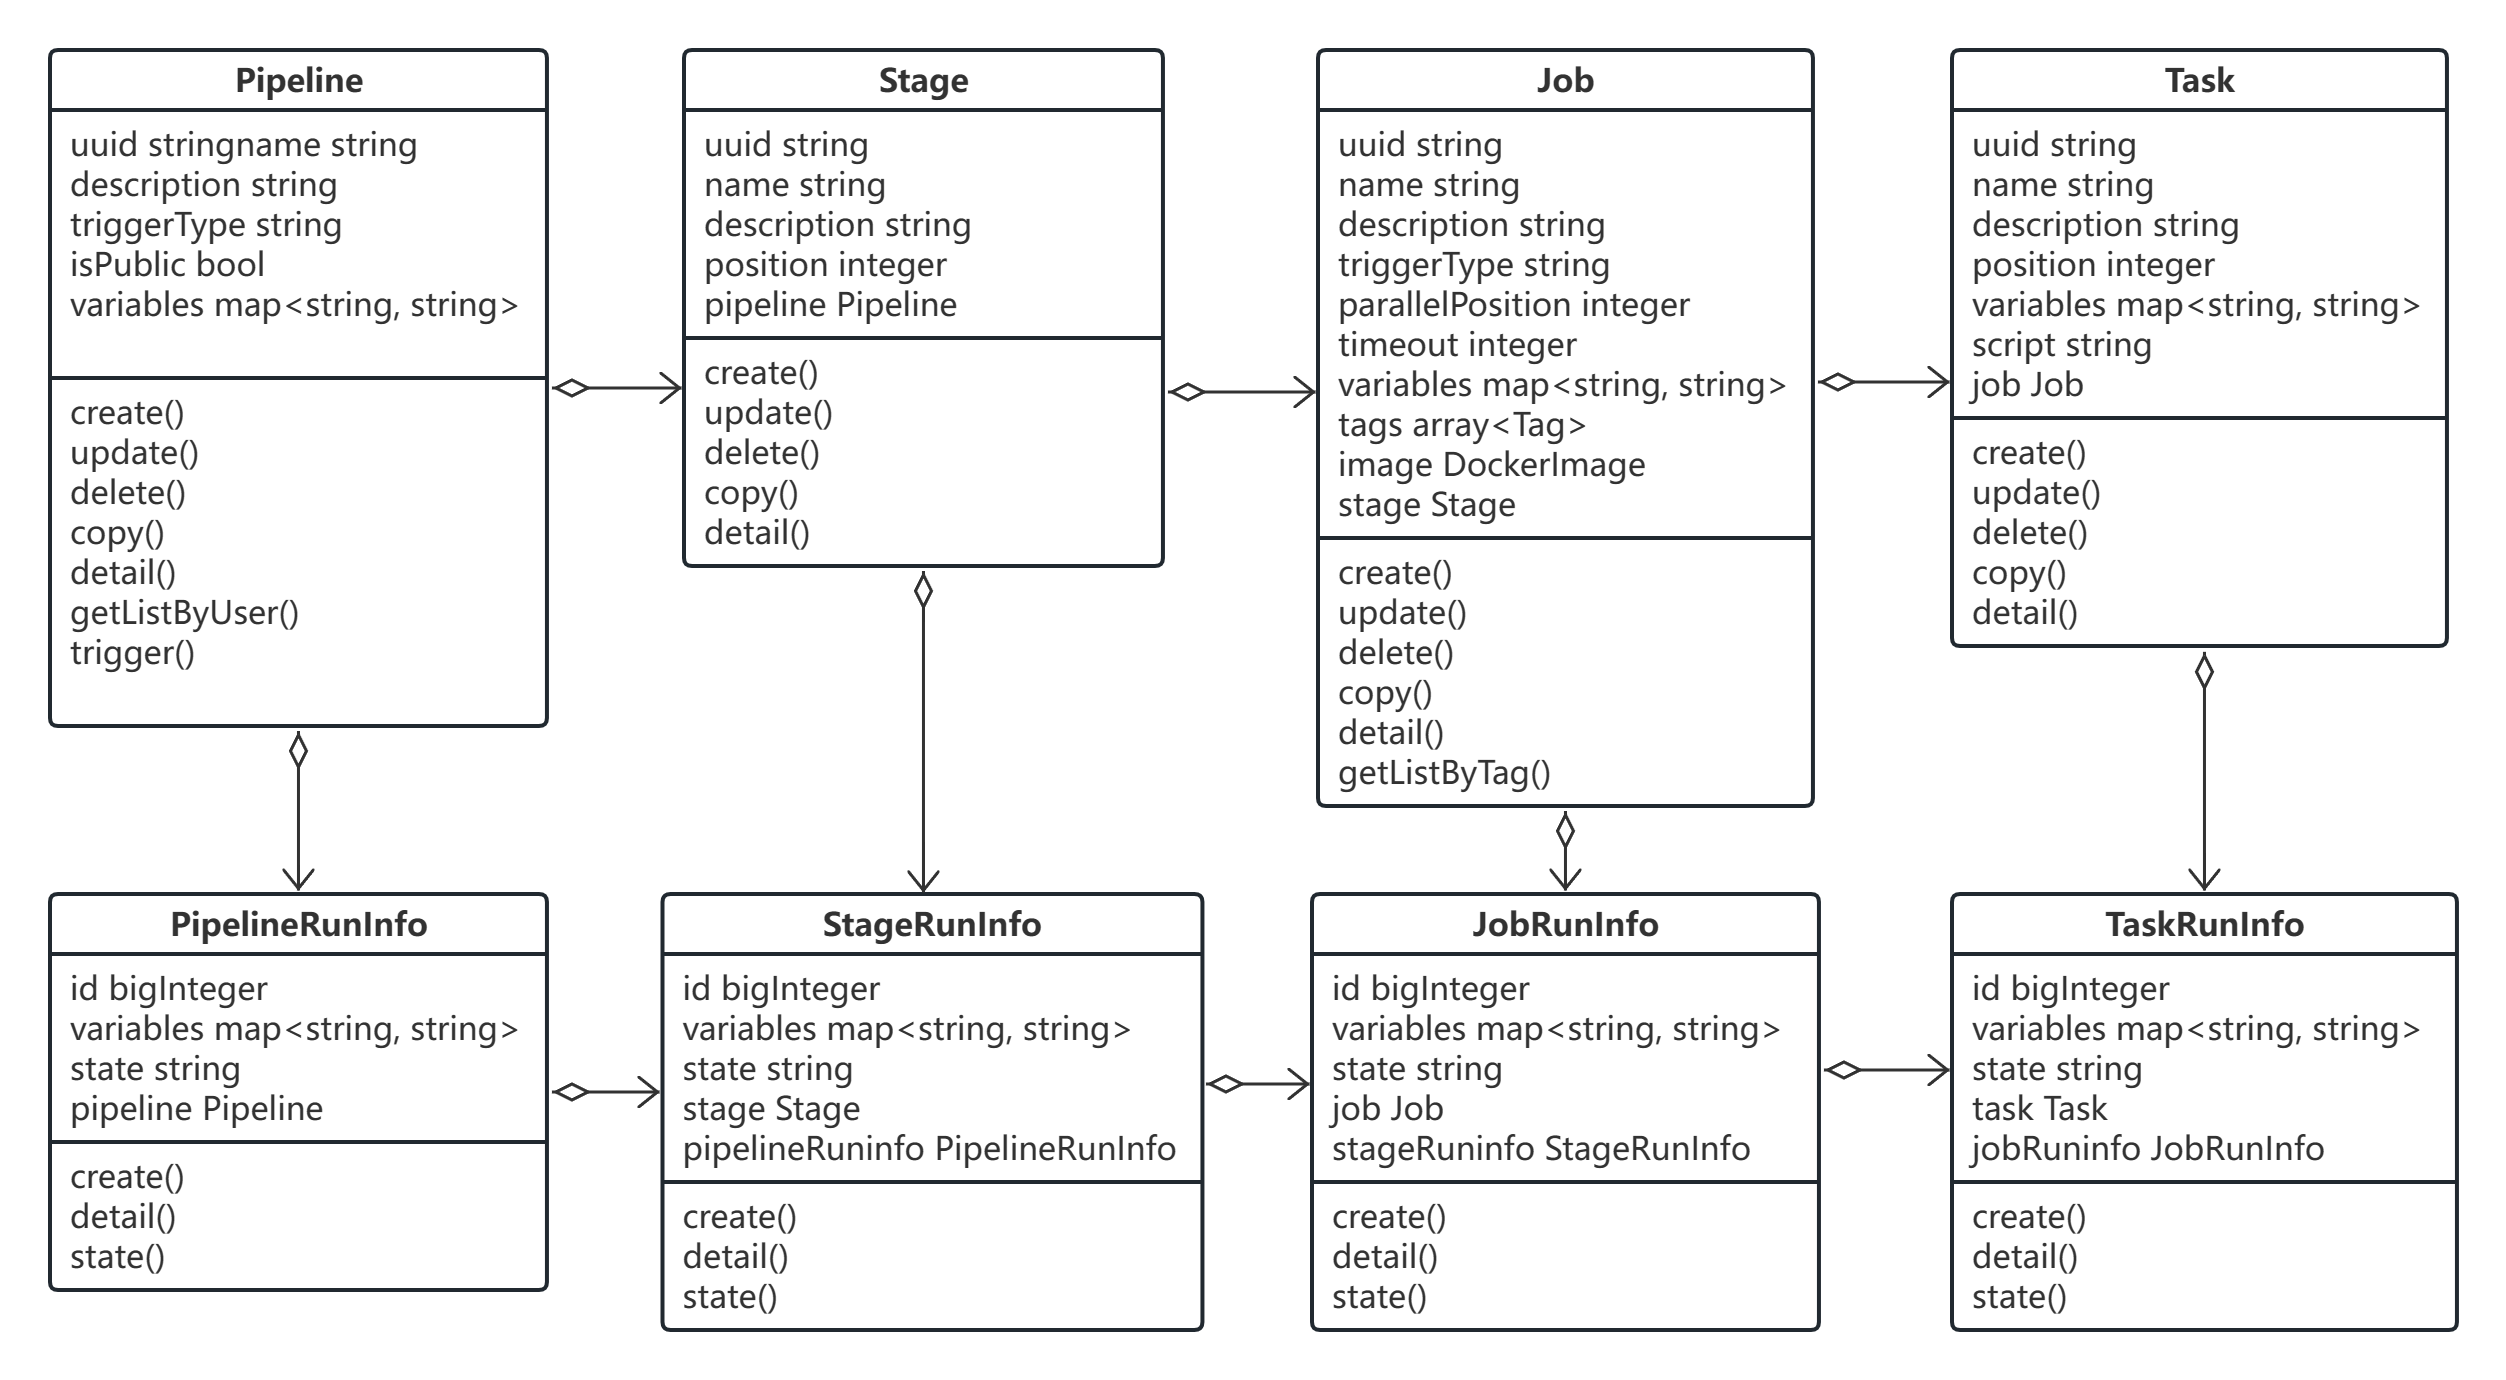
\includegraphics[width=1\textwidth]{流水线管理类图.png}
%   \caption{流水线管理类图}
%   \label{fig:流水线管理类图}
% \end{figure}

\section{镜像管理}
镜像管理的实现主要涉及到对Docker镜像及其操作的封装抽象,以及对Layer层的管理。类图如图\ref{fig:镜像管理类图}所示。

\begin{figure}[h]
  \centering
  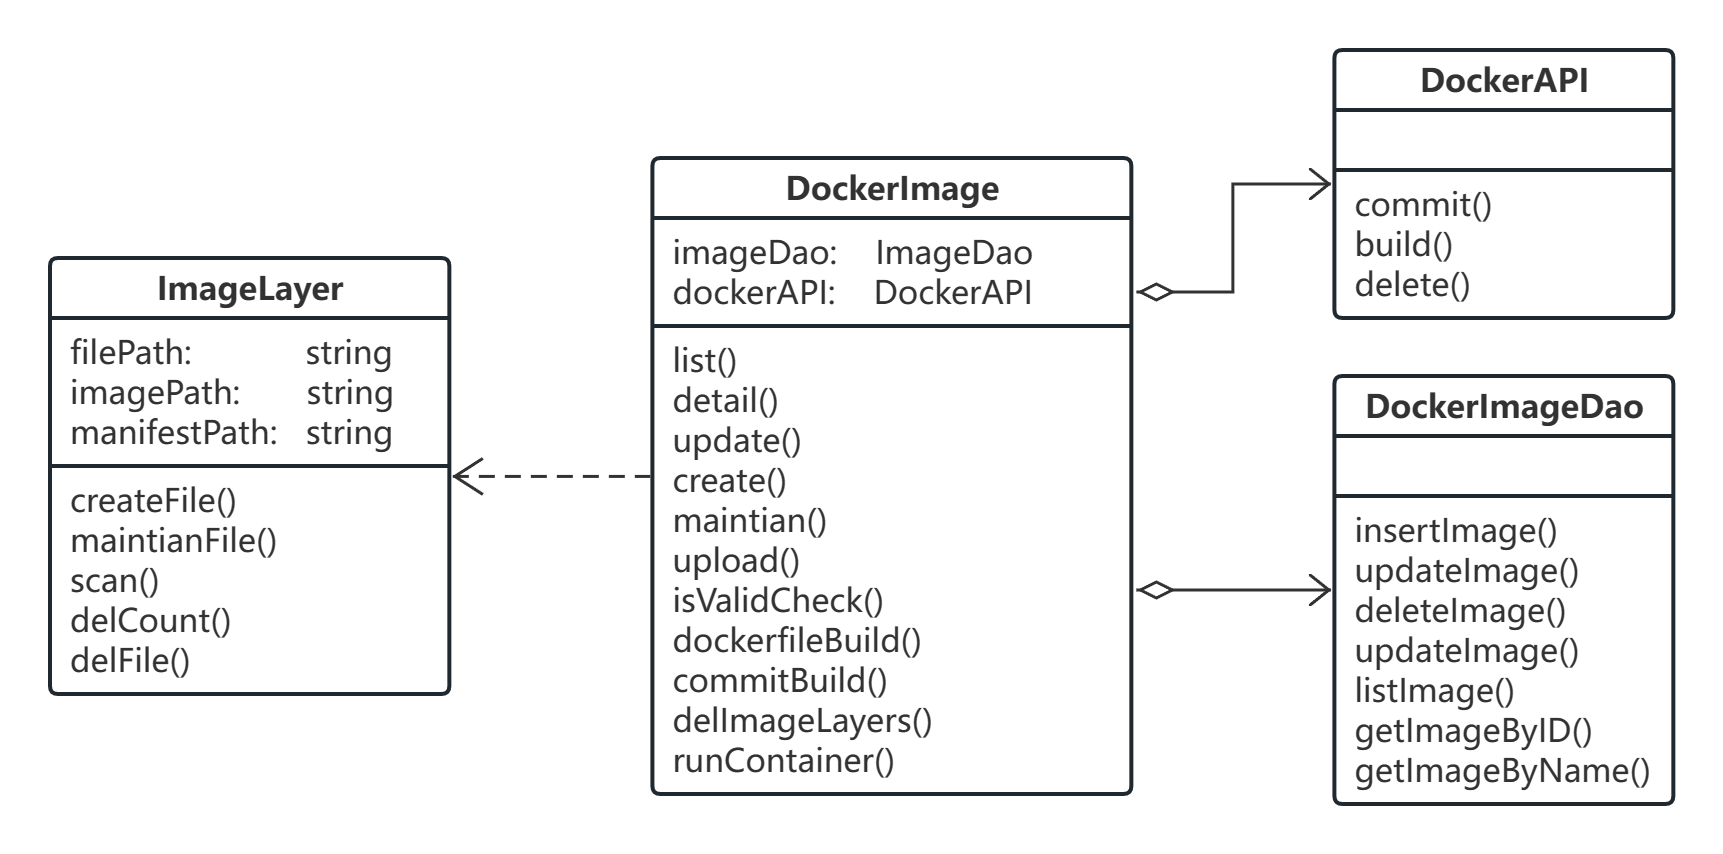
\includegraphics[width=1\textwidth]{镜像管理类图.png}
  \caption{镜像管理类图}
  \label{fig:镜像管理类图}
\end{figure}

\subsection{制作镜像}
制作镜像首先需要用户填写一系列基本信息,包括:镜像名称、镜像描述、镜像标签(Label)等,之后系统会实例化一个DockerImage类对象,
该类对象则包含了一些镜像的属性以及相应操作。

系统首先调用DockerImage.isValidCheck()来检测基础内容是否符合要求,如镜像名称是否有重复,镜像标签是否包含非法字符等。
然后,根据用户传入的制作选项,分别调用不同的制作策略:如果是Dockerfile的策略,系统将调用DockerImage.dockerfileBuild()方法并传入用户传入的文件,
方法内部将ssh进入系统的setting文件中配置的镜像制作服务器,执行docker build命令来直接构建镜像,最后将镜像传入镜像仓库;
如果是Commit策略则首先系统将调用DockerImage.commitBuild()方法,方法内部会在镜像服务器中根据用户配置的基础镜像,执行docker run来启动一个容器,并暴露出容器内部的ssh端口,
此后前端通过Wetty连接容器,此后用户便可以在用户界面使用终端进行操作。
注意,为了保证系统的安全性,我们需要对用户请求进行验证,如果不进行验证,当外部恶意模拟用户请求在服务器中创建容器,并通过一些手段影响到宿主机,会给系统带来极大的安全隐患。

\subsection{上传镜像}
根据在\nameref{subsec:镜像管理}中的分析,为了保证能够充分利用镜像仓库空间,确保不需要的镜像被完全删除,在镜像的上传和删除过程中均需要对Layer进行维护。
首先,前端发送上传镜像请求后,系统将调用DockerImage.upload()方法,该方法内部会判断DockerImage实例对象是否有label属性,根据label标签使用docker push命令推送至不同的仓库,如果没有标签则默认推送至公共仓库。

最后则需要进行Layer操作,首先实例化出ImageLayer实例,调用ImageLayer.scan()方法需要检测Layer文件是否存在,如果不存在则调用ImageLayer.createFile()方法,存在则调用ImageLayer.maintianFile()方法。

ImageLayer.createFile()和ImageLayer.maintianFile()方法会扫描Docker镜像的Manifest文件,将其中引用的ID与Layer实例的ID进行一一比较,从而判断Manifest文件中是否有引用该Layer,如果有则引用数加一,
如果没有则将Layer ID添加到引用文件中并设置引用值为1。这两个方法的区别在于ImageLayer.createFile()需要扫描所有的Manifest文件,而ImageLayer.maintianFile()只扫描指定的Manifest文件。

上传镜像时序图如图\ref{fig:上传镜像时序图}所示。

\begin{figure}[h]
  \centering
  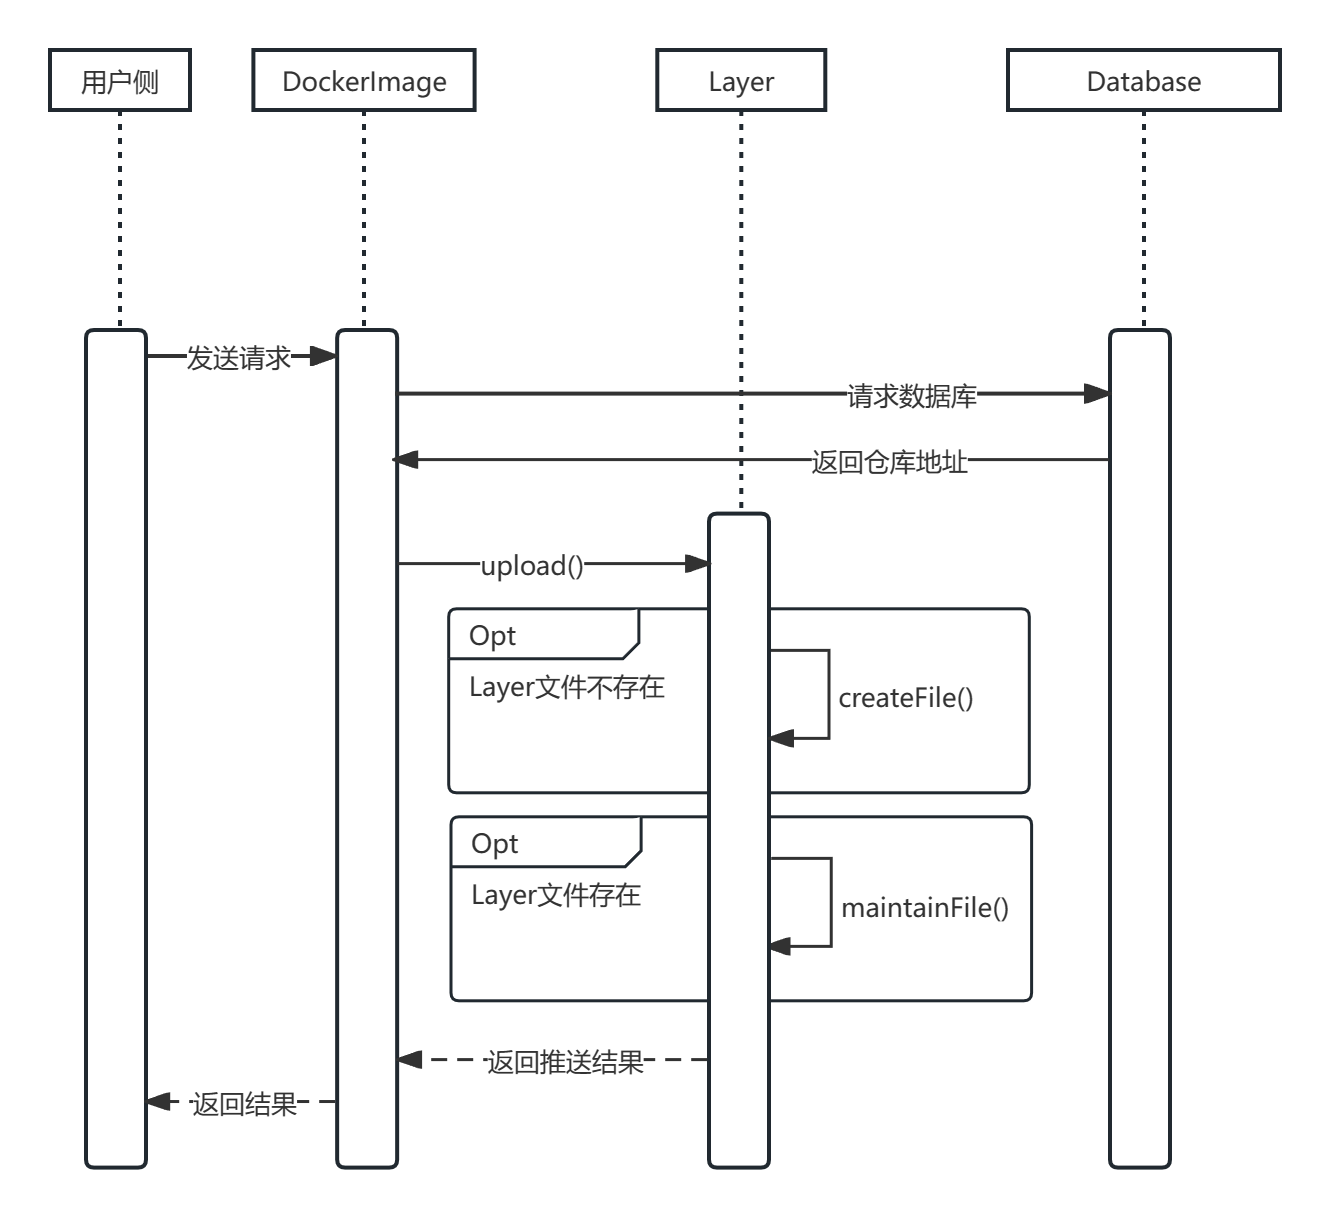
\includegraphics[width=1\textwidth]{上传镜像时序图.png}
  \caption{上传镜像时序图}
  \label{fig:上传镜像时序图}
\end{figure}

\subsection{删除镜像}
镜像由多个镜像层组成,并不是直接存储整个镜像本身,而是存储构成镜像的各个层。
对于每个Docker镜像,私有仓库利用一个Manifest配置文件来记录镜像所依赖的各层信息。当多个镜像共享同一层时,在仓库中该层只会被存储一次。
为解决以上问题,本模块优化了Docker官方的API,克服了无法移除底层文件的限制。这一过程主要包括两个阶段:首先扫描并移除不再需要的镜像层,然后利用Docker API删除相应的Manifest文件。

当需要删除特定镜像时,需对其引用的层进行移除。
我们通过DockerImage.delImageLayers()方法发起移除无效镜像层的请求。
鉴于可能有多个镜像引用同一层的情形,系统必须检查待删除的层是否还被其他镜像所引用。
直接检索每个镜像的Manifest文件以查找层引用会过于复杂,所以系统中为每个镜像层建立一个引用计数文件,记录层的ID和引用次数。
删除镜像时,相应层的引用计数减一。当某层的引用次数降至零时,系统将定位并直接删除该层对应的物理文件。
层的扫描、引用计数的减少及物理文件的删除分别由Layer.layerScan()、Layer.delCount()、Layer.delLayerFile()方法完成。

在移除引用计数文件和层文件之后,最后需调用Docker API来删除对应的Manifest文件,实现Manifest文件的最终删除。


\section{节点管理}



\subsubsection{节点一键部署}

\subsubsection{节点的上线与下线}


\section{插件市场}

\section{调度器的实现}

\subsection{状态转移模块的实现}

调度器中以状态机的设计模型来控制流水线中作业和任务的状态流转。
以下介绍作业状态机的详细设计,任务状态机与作业状态机极为相似,此处不再赘述。

按照有限状态机的设计理念,我们首先需要确定作业状态机的状态(State)和事件(Event)。
依据需求分析,系统中设计了以下作业状态:就绪中(Pending)、执行中(Running)、执行成功(Success)、执行失败(Failed)、被跳过(Skipped)和被取消(Canceled)。
同时设计了以下事件:触发(triggerEvent)、重试(retryEvent)、作业成功(successEvent)、作业失败(failEvent)、作业执行超时(timeoutEvent)、跳过(skipEvent)、取消(cancelEvent)、审核通过(reviewApproveEvent)和审核失败(reviewRejectEvent)。
依据状态机的设计模式,系统中将流水线作业的不同状态封装为类,将引起其状态转移的事件设置为成员方法。图~\ref{fig:作业状态机类图}为作业状态机类图。

\begin{figure}[h]
  \centering
  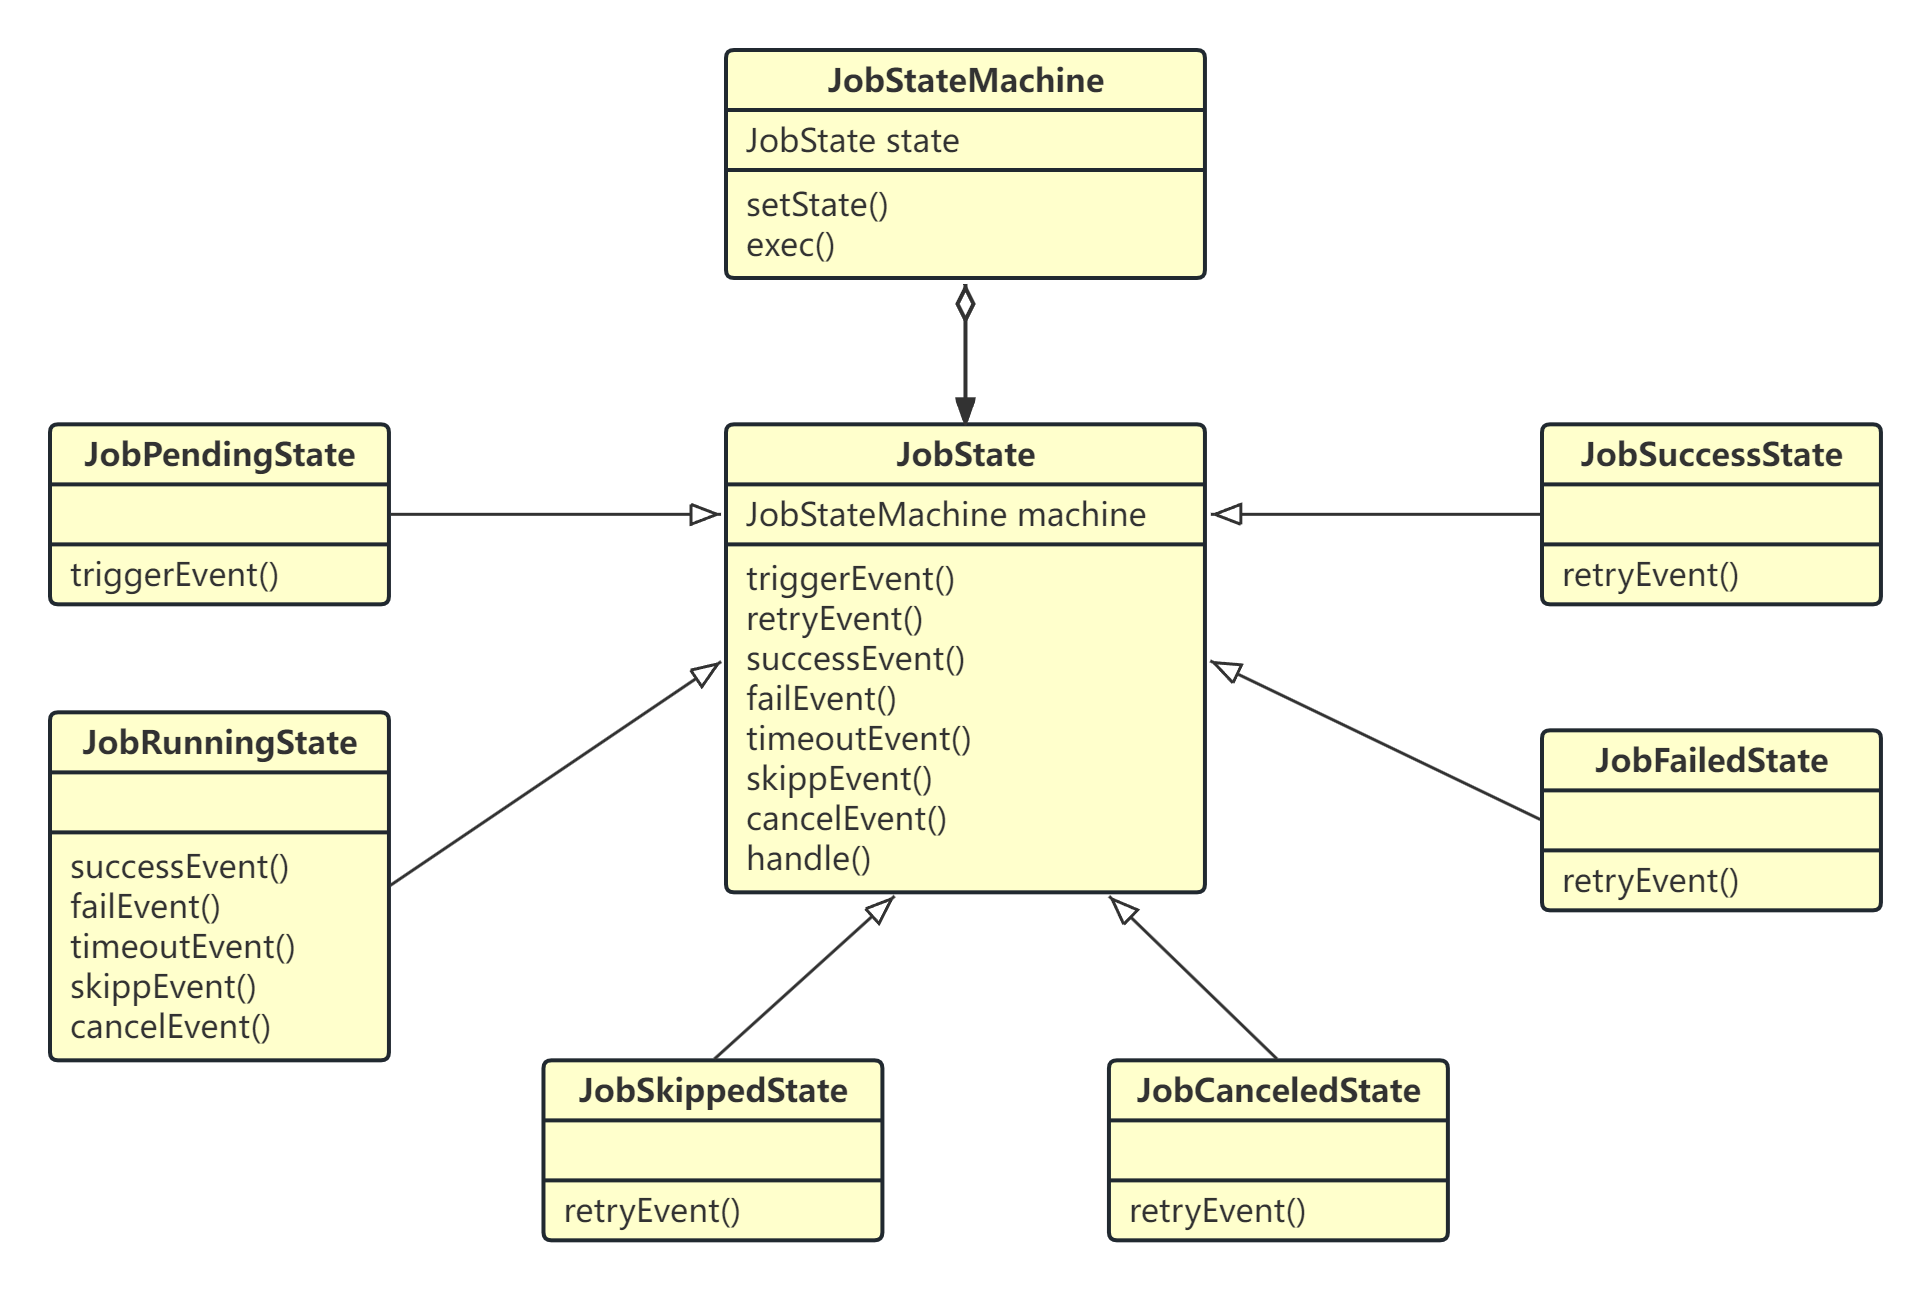
\includegraphics[width=1\textwidth]{作业状态机类图.png}
  \caption{作业状态机类图}
  \label{fig:作业状态机类图}
\end{figure}

当需要进行作业状态转换时,首先创建JobStateMachine实例并设置默认初始状态,然后向exec成员方法中传入当前发生的事件。
其中JobState是作业状态的抽象类,作业中每个具体的状态作为一个JobState的实现类,并从JobState中选择引起其状态转移的事件方法来实现。
例如JobRunningState类实现了JobState中的successEvent、failEvent、timeoutEvent、skippEvent和cancelEvent五个成员方法,这是因为这些事件均能作用于一个正在运行中的作业并且引起其状态改变,
其中successEvent方法会调用父类中持有的实例的JobStateMachine成员的setState方法,将当前状态机的状态设置为成功,并完成一些后续工作,其余事件方法也与之类似。

接下来具体分析作业状态机内部的状态转换:
当一个作业运行实例被创建时其应为就绪中状态,故就绪中(Pending)状态为初始状态,引发其状态改变的事件是触发(triggerEvent),这个触发事件是由决策中心经过决策逻辑发出的,并不只是用户的动触发行为,
一旦作业被成功触发,其状态则改变为运行中(Running);如果该作业被设定为需要人工审核才能触发,则审核通过事件(reviewApproveEvent)将会将状态改变为运行中(Running),审核驳回事件(reviewRejectEvent)将会将状态改变为失败(Failed)。
当作业处于运行中时,调度器可能会收到来自两方面的信号,其一是执行器所通知的作业执行状态,包括作业执行成功(successEvent)、执行失败(failEvent)和执行超时(timeoutEvent),
其中执行成功会使得作业状态机变为执行成功状态(Success),执行失败和执行超时都会变为执行失败状态(Failed);
其二是CI-Service所通知的用户人工干预命令,包括取消作业(cancelEvent)和跳过(skipEvent)作业,这两种事件会立即使得作业状态机变为取消(Canceled)和跳过(Skipped)状态。
以上两种信号均由决策中心先收到信号并统一处理决策后再转发给状态机,这样做可以统一外界信号的入口,降低其他模块与调度器间的耦合。
当处于运行中的作业进入终态后,作业仍然可以通过重试事件(retryEvent)来重新进入运行中的状态。
至于当前的作业是否满足触发该事件的条件,或者是否需要人工审核,由决策中心统一处理后发出信号,状态机不做额外的业务逻辑判断。

图~\ref{fig:流水线作业状态图}展示了作业状态机的状态流转。

\begin{figure}[h]
  \centering
  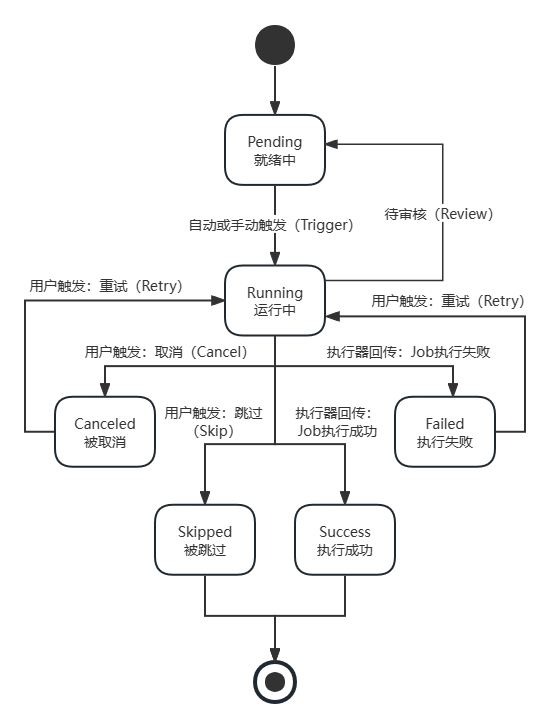
\includegraphics[width=0.7\textwidth]{流水线作业状态图.png}
  \caption{流水线作业状态图}
  \label{fig:流水线作业状态图}
\end{figure}

对于流水线和阶段的状态转移则相对比较简单。
对于阶段来讲,阶段的状态并不受到的具体的作业运行情况的影响,而是根据当前该阶段内所有作业的状态来综合决定,阶段状态机的类图如图\ref{}所示。

首先我们需要定义一套

\subsection{作业管理与决策中心模块的实现}

作业管理是调度器对Backend模块传入的作业信息进行二次封装和操作的模块。
决策中心则是整个调度器的核心模块,负责根据当前发生的事件(Event)和当前作业状态对作业管理模块中获得的作业进行决策。
作业管理与决策中心的类图如图\ref{fig:作业管理与决策中心类图}所示。

\begin{figure}[h]
  \centering
  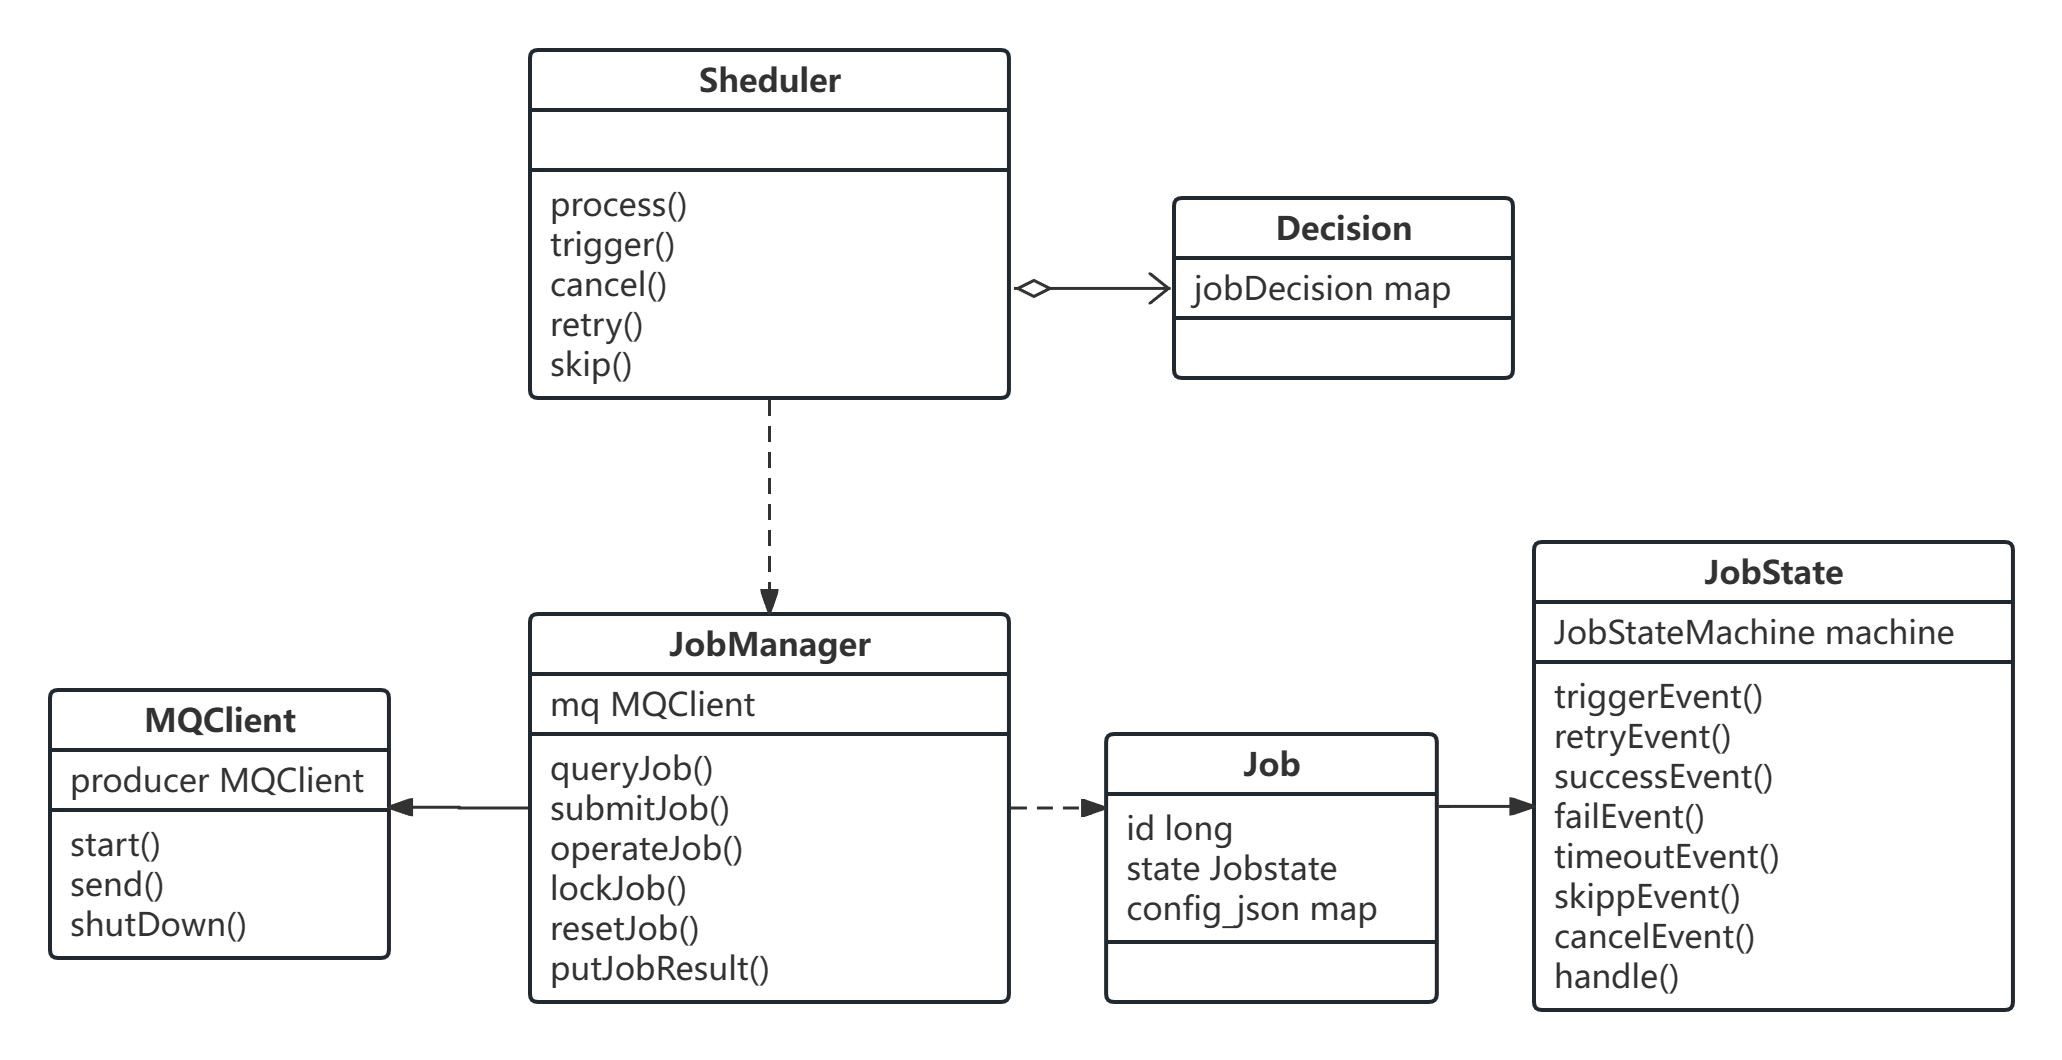
\includegraphics[width=1\textwidth]{作业管理与决策中心类图.png}
  \caption{作业管理与决策中心类图图}
  \label{fig:作业管理与决策中心类图}
\end{figure}

调度器模块的架构细节展现在图 3.13 中。Scheduler 类位于调度模块的核心位置,其主要负责执行一个关键功能:processTask。该方法的主要职责是从作业管理器中拉取待处理的作业,并基于作业事件及其当前状态来做出相应的调度决策。makeRunDecision方法体现了该决策逻辑,而当决策包含特定的作业处理时,batchPutJobDecision则被用于执行相关操作。决策对象由Decision类封装,其中作业的决策以Map形式存在,以便支持作业的并行处理能力。DecisionEnum枚举了可能的决策事件,这些事件直接影响流水线作业和作业状态的转换。

作业管理(JobManager)和Scheduler交互是通过作业实体Job进行的,其中JobManager类似于TaskCenter,但专注于作业层面的管理。与TaskCenter类似,putJobResult方法接受执行器返回的状态更新,并将相关作业重新排队等待下一轮调度决策。getUnackJobs方法能够查询那些已经分发给执行器但尚未执行的作业。

调度器的执行逻辑在图 3.14 的时序图中有详细展示。系统初始化时,Scheduler.process()方法将在守护线程中运行,不断地处理作业。当Backend服务接收到用户发起的流水线事件时,会通过addJob()方法将作业提交至消息队列中进行排队。
此处需要注意,由于系统中调度器是多实例部署,属于分布式系统,任何一个节点都有可能处理这些作业,如此便产生了竞态条件,为了避免发生无法预期的错误,
以及保证作业不丢失,在进行决策前,必须通过JobManager.lockJob()方法对作业加锁,以获得处理权。

Scheduler在接收到一批待处理作业后,会根据每个作业的具体事件类型及其包含的状态进行详细决策。
完成决策后,决策结果Decision将被检查,如果包含对作业的决策,则将其发送回作业管理器以便进一步处理,这可能会导致作业状态的变更,则交由JobStateMachine进行处理。
若决策中未包含对整个作业的处理,而是针对特定作业的,则会触发作业管理器的相关处理逻辑,并通过后端服务进行状态持久化。

结合以上内容,作业调度时序图如图\ref{fig:作业调度时序图}所示。

\begin{figure}[h]
  \centering
  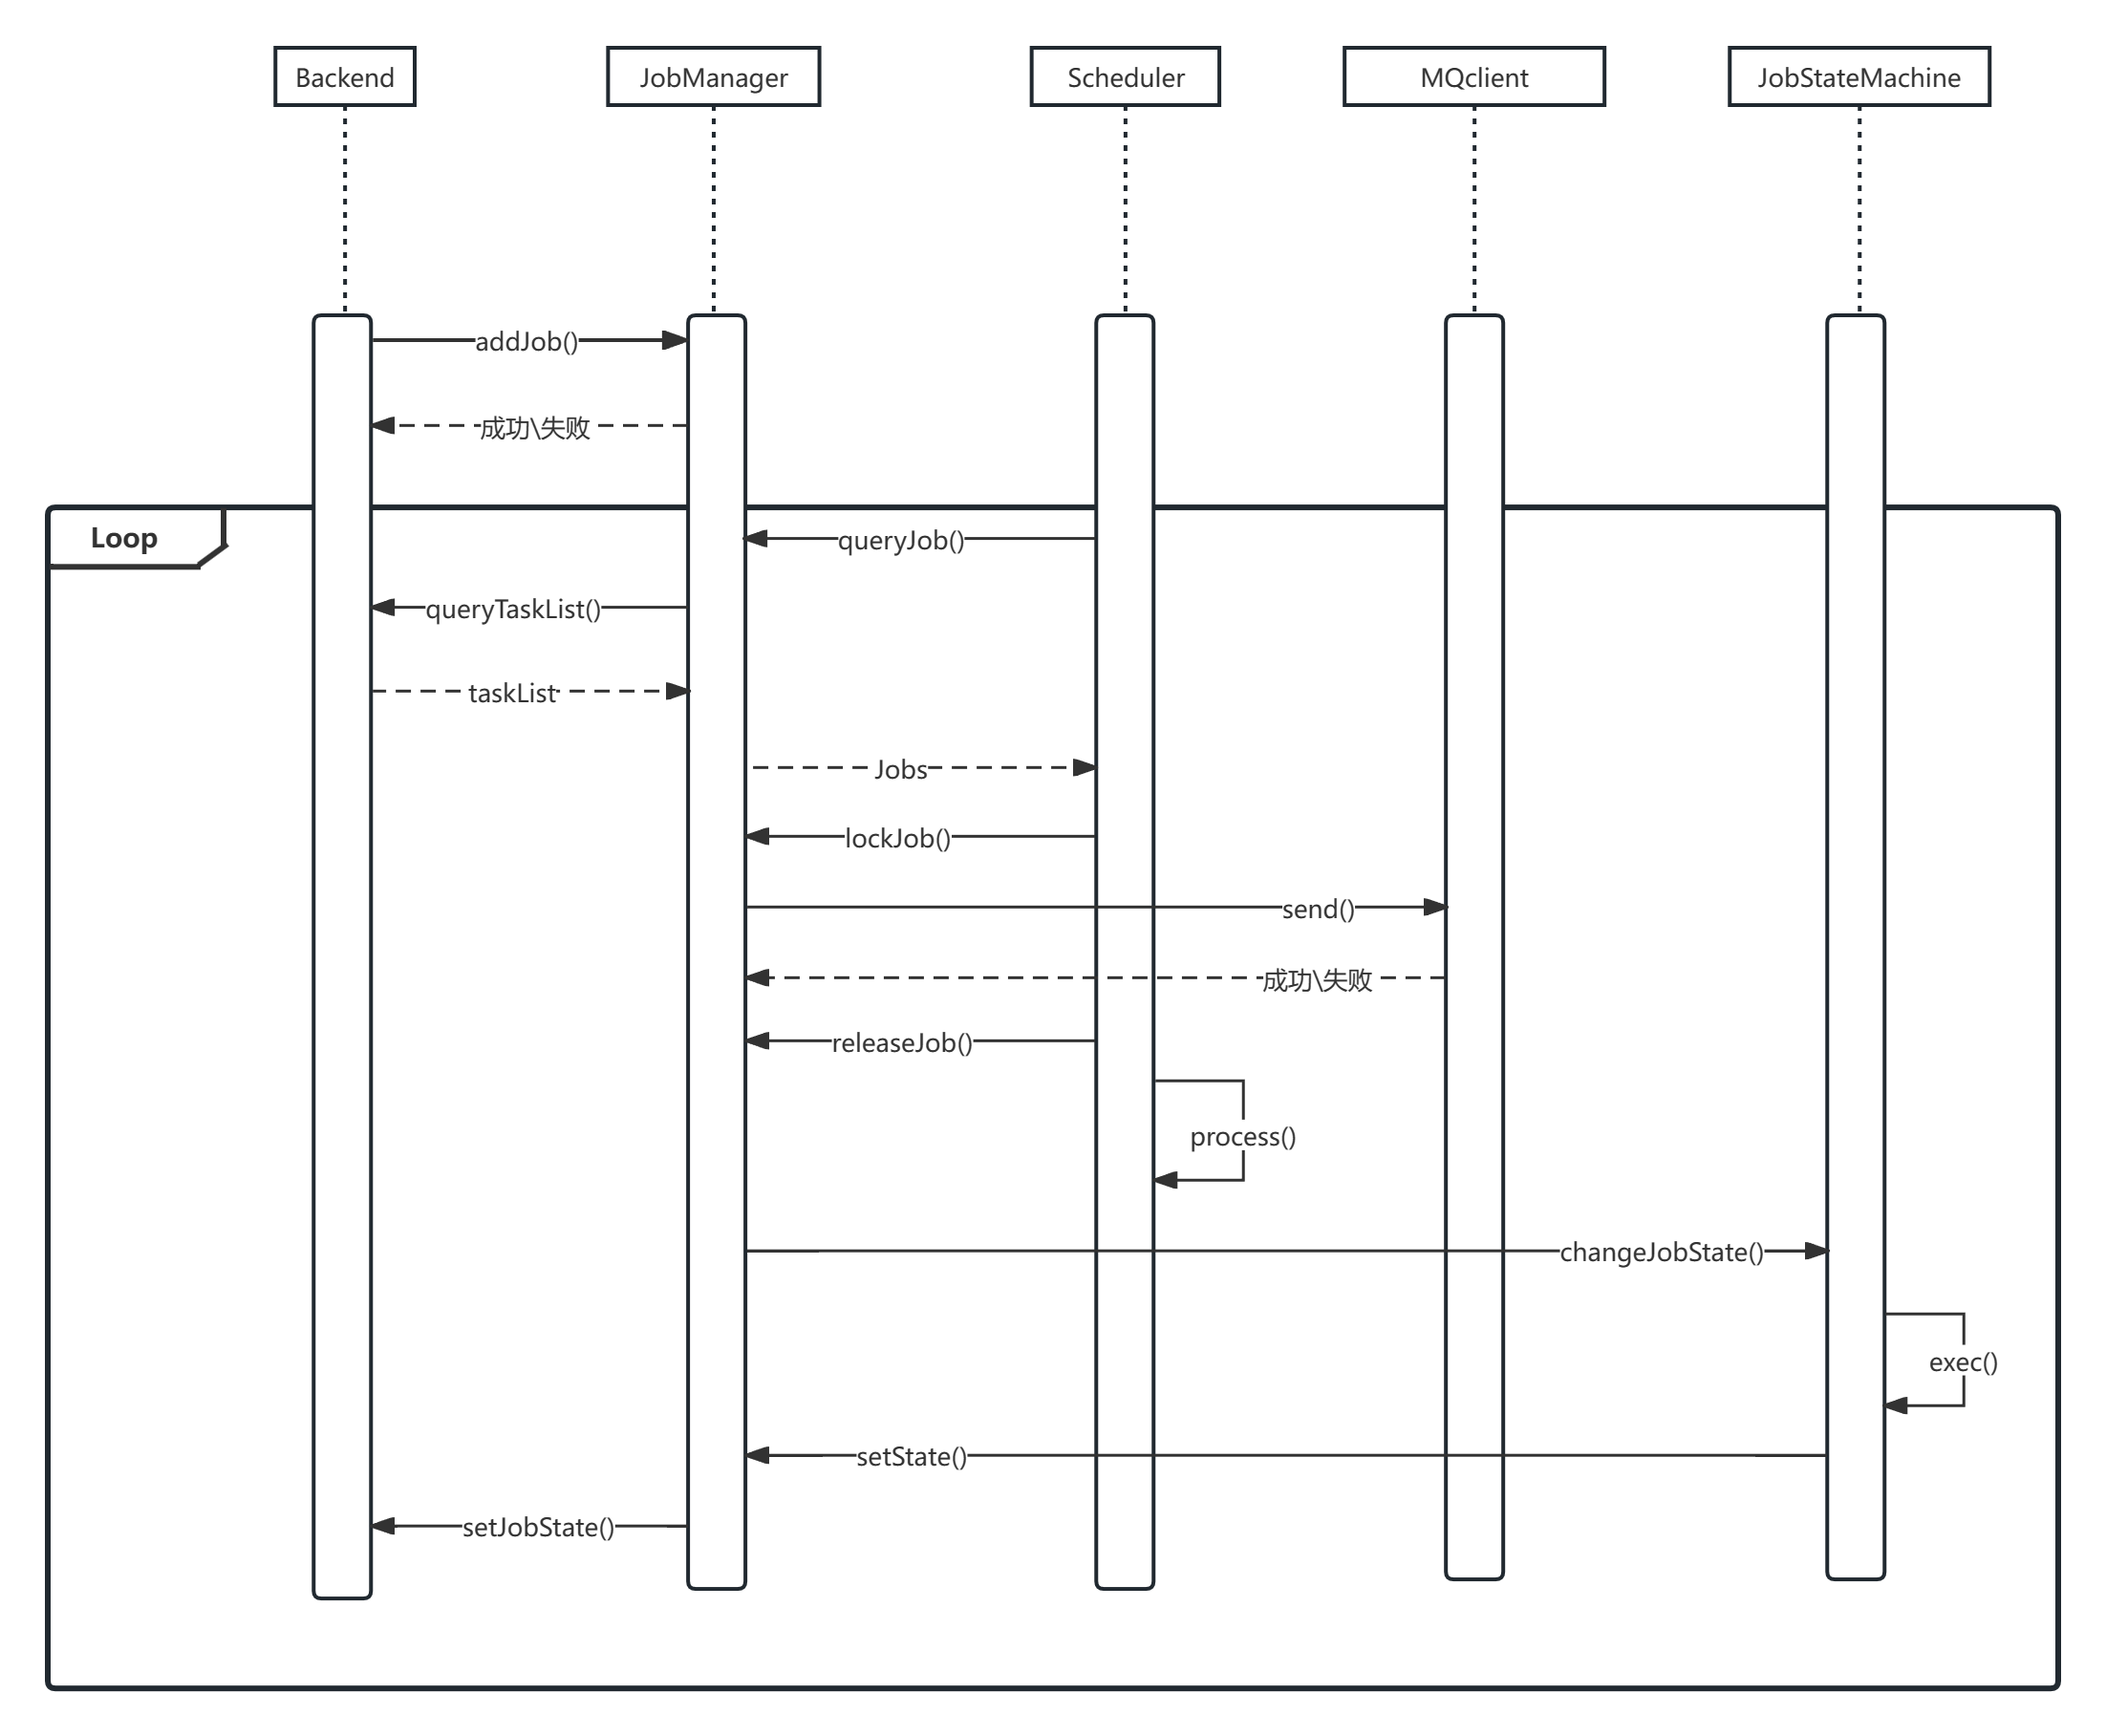
\includegraphics[width=1\textwidth]{作业调度时序图.png}
  \caption{作业调度时序图}
  \label{fig:作业调度时序图}
\end{figure}

